\documentclass{article}
\usepackage{tikz}

\begin{document}

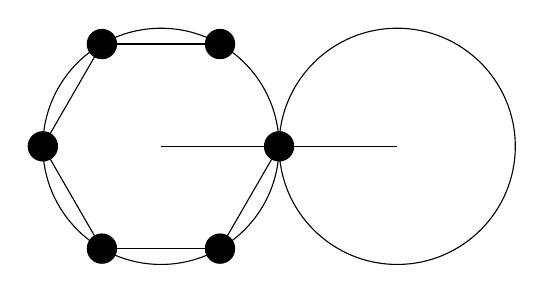
\begin{tikzpicture}[scale=1.5]
  % Define the circles
  \draw (0,0) circle (1);
  \draw (2,0) circle (1);

  % Define the vertices
  \foreach \i in {1,...,6} {
    \pgfmathsetmacro{\angle}{360/6 * (\i - 1)}
    \node[circle,fill=black,inner sep=1pt] at (\angle:1) {\i};
  }

  % Draw the connecting lines
  \draw (0,0) -- (2,0);
  \foreach \i in {1,...,6} {
    \pgfmathtruncatemacro{\nexti}{mod(\i+1,7)}
    \draw (\i*60:1) -- (\nexti*60:1);
  }
\end{tikzpicture}

\end{document}